% CVPR 2022 Paper Template
% based on the CVPR template provided by Ming-Ming Cheng (https://github.com/MCG-NKU/CVPR_Template)
% modified and extended by Stefan Roth (stefan.roth@NOSPAMtu-darmstadt.de)

\documentclass[10pt,twocolumn,letterpaper]{article}

%%%%%%%%% PAPER TYPE  - PLEASE UPDATE FOR FINAL VERSION %%%%%%%%%
%\usepackage[review]{cvpr}      % To produce the REVIEW version
%\usepackage{cvpr}              % To produce the CAMERA-READY version
\usepackage[pagenumbers]{cvpr} % To force page numbers, e.g. for an arXiv version

% Include other packages here, before hyperref.
\usepackage{graphicx}
\usepackage{amsmath}
\usepackage{amssymb}
\usepackage{booktabs}
\usepackage{float}
\usepackage{arydshln}


% It is strongly recommended to use hyperref, especially for the review version.
% hyperref with option pagebackref eases the reviewers' job.
% Please disable hyperref *only* if you encounter grave issues, e.g. with the
% file validation for the camera-ready version.
%
% If you comment hyperref and then uncomment it, you should delete
% ReviewTempalte.aux before re-running LaTeX.
% (Or just hit 'q' on the first LaTeX run, let it finish, and you
%  should be clear).
\usepackage[pagebackref,breaklinks,colorlinks]{hyperref}


% Support for easy cross-referencing
\usepackage[capitalize]{cleveref}
\crefname{section}{Sec.}{Secs.}
\Crefname{section}{Section}{Sections}
\Crefname{table}{Table}{Tables}
\crefname{table}{Tab.}{Tabs.}

\begin{document}

%%%%%%%%% TITLE - PLEASE UPDATE %%%%%%%%%
\title{VRDL HW4: Image Restoration Report}

\author{Yi-Hsiang Ho, 111550106
% For a paper whose authors are all at the same institution,
% omit the following lines up until the closing ``}''.
% Additional authors and addresses can be added with ``\and'',
% just like the second author.
% To save space, use either the email address or home page, not both
% \and
% Second Author\\
% Institution2\\
% First line of institution2 address\\
% {\tt\small secondauthor@i2.org}
}
\maketitle

%%%%%%%%% BODY TEXT %%%%%%%%%

% ------------------------- Introduction -------------------------

\section{Introduction}
\label{sec:intro}

This task involves image restoration, especially for two types of degradations ---
Derain and Desnow, using PromptIR~\cite{PromptIR}. The dataset has 3,200 paired
images, with degradation and the corresponding clean images, for training. Both
deraining and desnowing task each have 1,600 images, and the degraded types
are labeled as well. It also provides 100 images, without degraded type notations,
for testing.

The core idea of this work is to change the loss functions to cover more
aspects of the clean image, apply test-time augmentation (TTA) to improve
performance, and ensemble multiple models to achieve better results. The
implementation is based on the official codebase of PromptIR~\cite{PromptIR}.
GitHub repository is available
\href{https://github.com/Sean20405/NYCU-DLVR-HW4}{here}.

\subsection{Image Restoration}

Image restoration aims to recover high-quality images from degraded observations,
often caused by noise, blur, or environmental factors. Among these tasks,
deraining and desnowing are critical for improving visibility and performance
in outdoor vision systems. Rain and snow streaks introduce complex, spatially
varying distortions that challenge traditional restoration methods.

\begin{figure}[h]
  \centering
  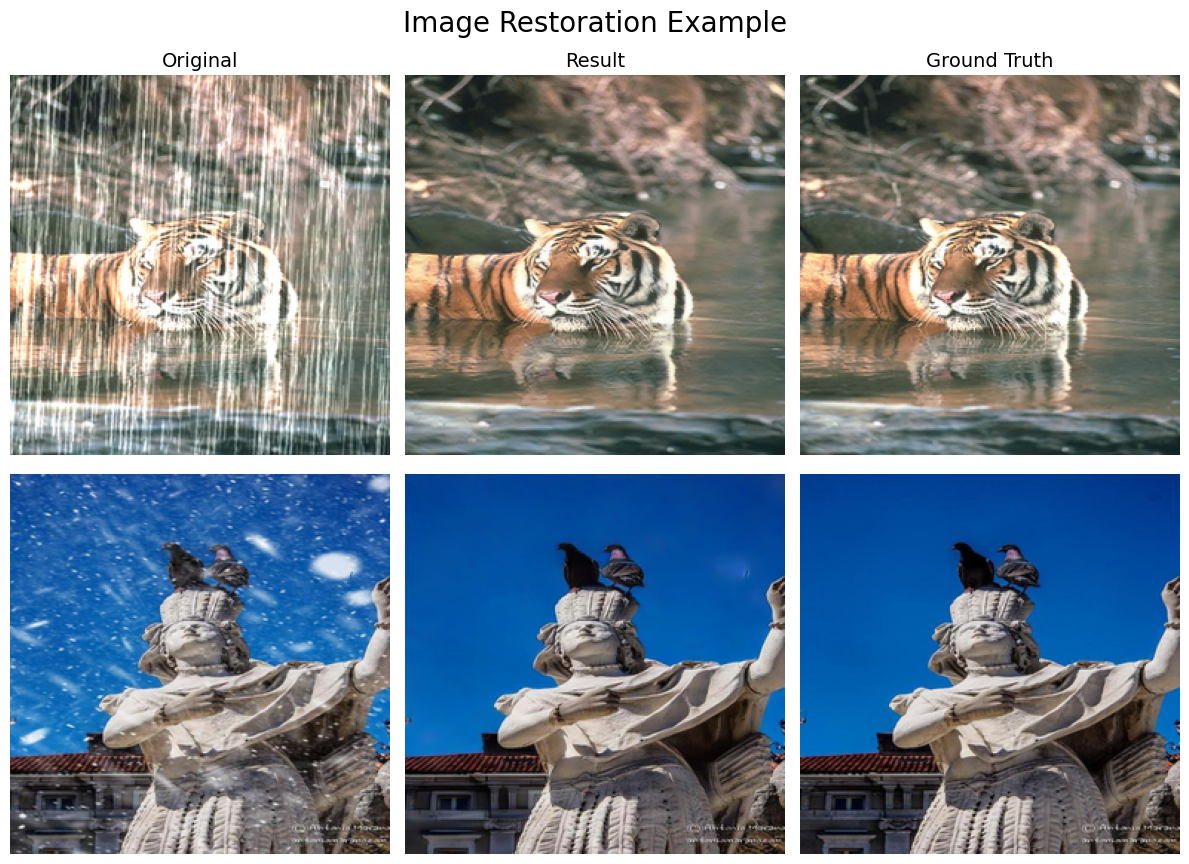
\includegraphics[width=0.95\linewidth]{assets/image_restoration.png}
  \caption{\textbf{The image restoration task.} The first row is deraining task,
    while the second row is desnowing task.}
  \label{fig:image_restoration}
\end{figure}

\subsection{PromptIR}

PromptIR~\cite{PromptIR} is a novel framework for blind image restoration that
leverages prompt-based learning to adaptively handle various image degradations
without requiring explicit degradation labels. By introducing learnable prompts
into a frozen image restoration backbone, PromptIR enables flexible and
efficient restoration across diverse tasks such as denoising, deblurring, and
super-resolution. This approach significantly reduces training costs while
maintaining high performance, highlighting the potential of prompt tuning in
generalizing image restoration models across different degradation types.

\subsection{Test-Time Augmentation}

Test-time augmentation (TTA) is a technique used to enhance model performance
during inference by applying various transformations, such as flipping, rotation,
or scaling, to input images. The model generates predictions for each augmented
version, which are then averaged to produce a more robust final output.

\subsection{Ensemble Learning}

Ensemble learning combines multiple models to improve performance. It averages
the predictions of multiple models to make the final prediction. This technique
helps to reduce variance, increase accuracy, and improve model robustness.


% --------------------------- Method ---------------------------

\section{Method}
\label{sec:method}

\subsection{Data Preprocessing and Augmentation}
\label{subsec:aug}

The training dataset contains 3,200 degraded images with corresponding clean
images. It is split into training and validation sets with a ratio of 8:2.

Some data augmentations are applied to the training set. These include:
\begin{itemize}
  \setlength\itemsep{0pt}
  \item Random horizontal flip
  \item Random vertical flip
  \item Random rotation
  \item Random cropping
\end{itemize}

\subsection{Model Architecture}

The model follows the same architecture as PromptIR~\cite{PromptIR}, and the pipeline
is shown in \cref{fig:pipeline}. It uses a U-Net style architecture to perform
image restoration. An additional Prompt block is added to the model. It consists of a
prompt generation module (PGM) and a prompt interaction module (PIM). The prompt
generation module generates a prompt based on the latent $F_{p}$ from input image
and prompt components, which is a learnable parameter. The prompt interaction module
aims to integrate the prompt into the U-Net pipeline. The ``Prompt'' is injected
only into decoder part of the U-Net.

\begin{figure}[h]
  \centering
  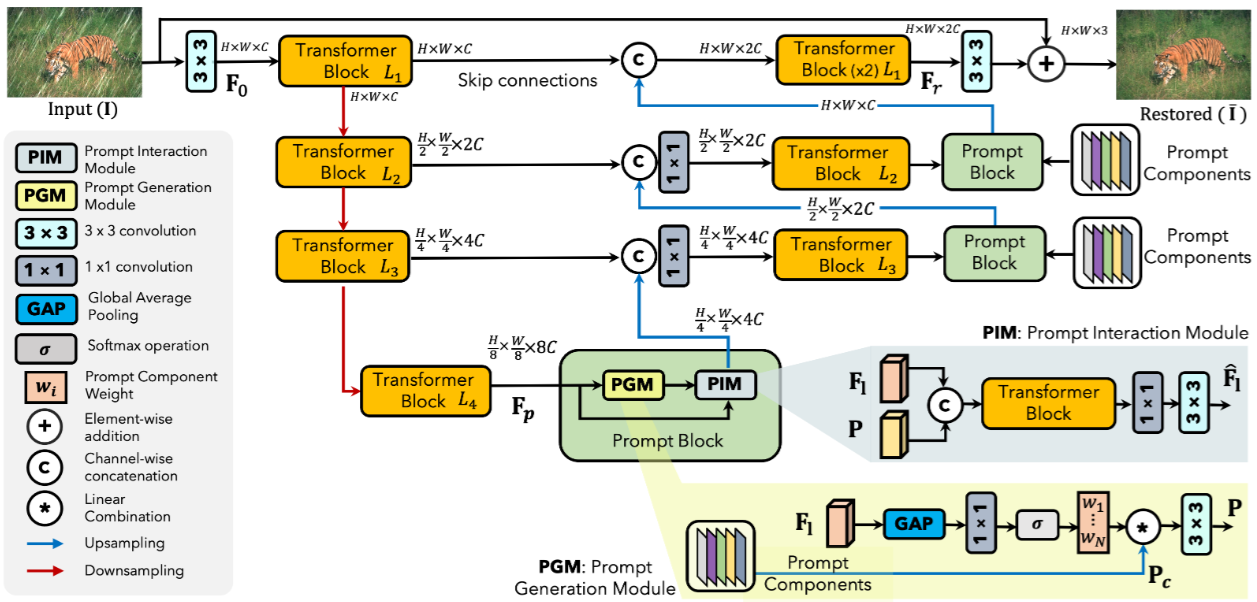
\includegraphics[width=0.95\linewidth]{assets/PromptIR_pipeline.png}
  \caption{\textbf{The pipeline of PromptIR.} (retrieved from
    PromptIR~\cite{PromptIR})}
  \label{fig:pipeline}
\end{figure}

\subsection{Loss Function}

The loss function is a combination of three losses: MSE loss
$\mathcal{L}_{2}$, edge loss $\mathcal{L}_{\text{edge}}$, and
perceptual loss $\mathcal{L}_{\text{vgg}}$, while the original implementation
only uses L1 loss. The MSE loss is used to measure the pixel-wise difference
between the predicted and ground truth images. The edge loss is to make the
model learn the edges of the objects in the image. It is calculated by applying
Sobel filter to the predicted and ground truth images, and then calculating the
L1 loss between the two edge maps. The perceptual loss is calculated by passing
the predicted and ground truth images through a pretrained VGG-16
network~\cite{VGG} and calculating the MSE loss between the feature maps of the
two images. The final loss is computed as follows:
\begin{equation}
  \mathcal{L} = \lambda_1 \cdot \mathcal{L}_{2} + \lambda_2 \cdot \mathcal{L}_{\text{edge}} + \lambda_3 \cdot \mathcal{L}_{\text{vgg}}
\end{equation}
where $\lambda_1$, $\lambda_2$, and $\lambda_3$ are hyperparameters that control
the contribution of each loss term. In this task, I set $\lambda_1 = 5.0$,
$\lambda_2 = 0.1$, and $\lambda_3 = 0.001$.

\subsection{Optimization}

For optimization, AdamW~\cite{AdamW} is used with an initial learning rate of 2e-4.
A linear warmup cosine annealing scheduler~\cite{LightningSched} dynamically adjusts
the learning rate throughout training. The choice of optimizer and scheduler follows
the same approach in original PromptIR. The training process is conducted with a batch
size of 4 over 300 epochs. The dataset contains 2,560 training images, 640 validation
images, and 100 testing images. The best-performing model is selected based on PSNR,
which is calculated on validation dataset. The model is trained on a single NVIDIA
GeForce RTX 4090 GPU in about 10 hours. 

\subsection{Inference}
\label{subsec:inference}

Test-time augmentation (TTA) is applied to the model during inference. The
model generates predictions for each augmented version of the input image,
which includes horizontal flip, vertical flip, and horizontal+vertical flip.
The final output is obtained by averaging the predictions of all augmented
versions.

Ensemble learning is also applied during inference. Three models trained with
different methods are used to generate predictions. The final output
is obtained by averaging the predictions of all models. That is, there are in total
4 x 3 = 12 predictions for each image, 4 images for TTA on each model and 3 models
selected for ensemble. The three models are:
\begin{itemize}
  \setlength\itemsep{0pt}
  \item Using $\mathcal{L}_{2}$ and $\mathcal{L}_{\text{edge}}$
    as loss function, without $\mathcal{L}_{\text{vgg}}$ and augmentation
  \item Using all three loss functions, without augmentation
  \item Using all three loss functions, with augmentation
\end{itemize}

\subsection{Hyperparameters}

\noindent The hyperparameter details are listed below:
\begin{itemize}
  \setlength\itemsep{0pt}
  \item Learning rate: 2e-4
  \item Optimizer: AdamW~\cite{AdamW}
  \item Scheduler: Linear warmup cosine annealing~\cite{LightningSched}
  \item Batch size: 4
  \item Epochs: 300
  \item Patch size: 128
  \item Loss weights: $\lambda_1 = 5.0$, $\lambda_2 = 0.1$, $\lambda_3 = 0.001$
\end{itemize}

\section{Results}

In this section, I compare the performance of each component in the model.
The details of each method are listed:
\begin{itemize}
  \setlength\itemsep{0pt}
  \item PromptIR: The original PromptIR model without any modification.
  \item Aug.: PromptIR + augmentation mentioned in \cref{subsec:aug}
  \item Loss w/o VGG: PromptIR with the loss function
    $\mathcal{L}_{2}$ and $\mathcal{L}_{\text{edge}}$, without
    $\mathcal{L}_{\text{vgg}}$.
  \item Loss: PromptIR with all loss function.
  \item TTA: ``Loss" with TTA
  \item Ensemble: Ensemble of three models mentioned in \cref{subsec:inference}.
\end{itemize}

The results are shown in \cref{tab:result}. The validation PSNR curve and loss
curve are shown in \cref{fig:val-psnr} and \cref{fig:val-loss}, respectively.
Each component improves the performance of PromptIR in testing dataset. TTA and
ensemble have a significant improvement. The loss for ``Loss'' is relatively
higher since the perceptual loss is not converged yet (see \cref{fig:val-perceptual}).
However, it still performs better than the original PromptIR model.

\begin{table}[h]
  \centering
  \begin{tabular}{lccc}
    \toprule
    \multicolumn{1}{c}{\textbf{Method}} & \textbf{Val}              & \textbf{Test pub.}          & \textbf{Test priv.} \\
    \midrule
    PromptIR                            & 28.9600                   & 30.1508                     & 29.3773             \\
    \hdashline
    Aug.                                & \tbbgblue 29.2972         & \tbbgred 30.0079            & \tbbgblue 29.3440   \\
    Loss w/o VGG                        & \tbbgblue 29.6007         & \tbbgblue 30.3480           & \tbbgblue 29.6707    \\
    Loss                                & \tbbgred 28.7450          & \tbbgblue 30.2550           & \tbbgblue 29.6516    \\
    TTA                                 & -                         & \tbbgblue 30.5405           & \tbbgblue 29.7865    \\       
    Ensemble                            & -                         & \tbbgblue \textbf{30.7608}  & \tbbgblue \textbf{30.0588} \\
    \bottomrule
  \end{tabular}
  \caption{\textbf{The PSNR results of different methods.} ``Val" refers to
    validation PSNR. ``Test pub." and ``Test priv." refer to public and
    private test set PSNR, respectively. PromptIR is treated as the baseline.
    If the value is higher than PromptIR, it is highlighted in blue, or it will
    be in red. The highest values in each column are also highlighted in bold.
    TTA and Ensemble are not evaluated in validation set, so the values are
    not available.
  }
  \label{tab:result}
\end{table}

\begin{figure}[h]
  \centering
  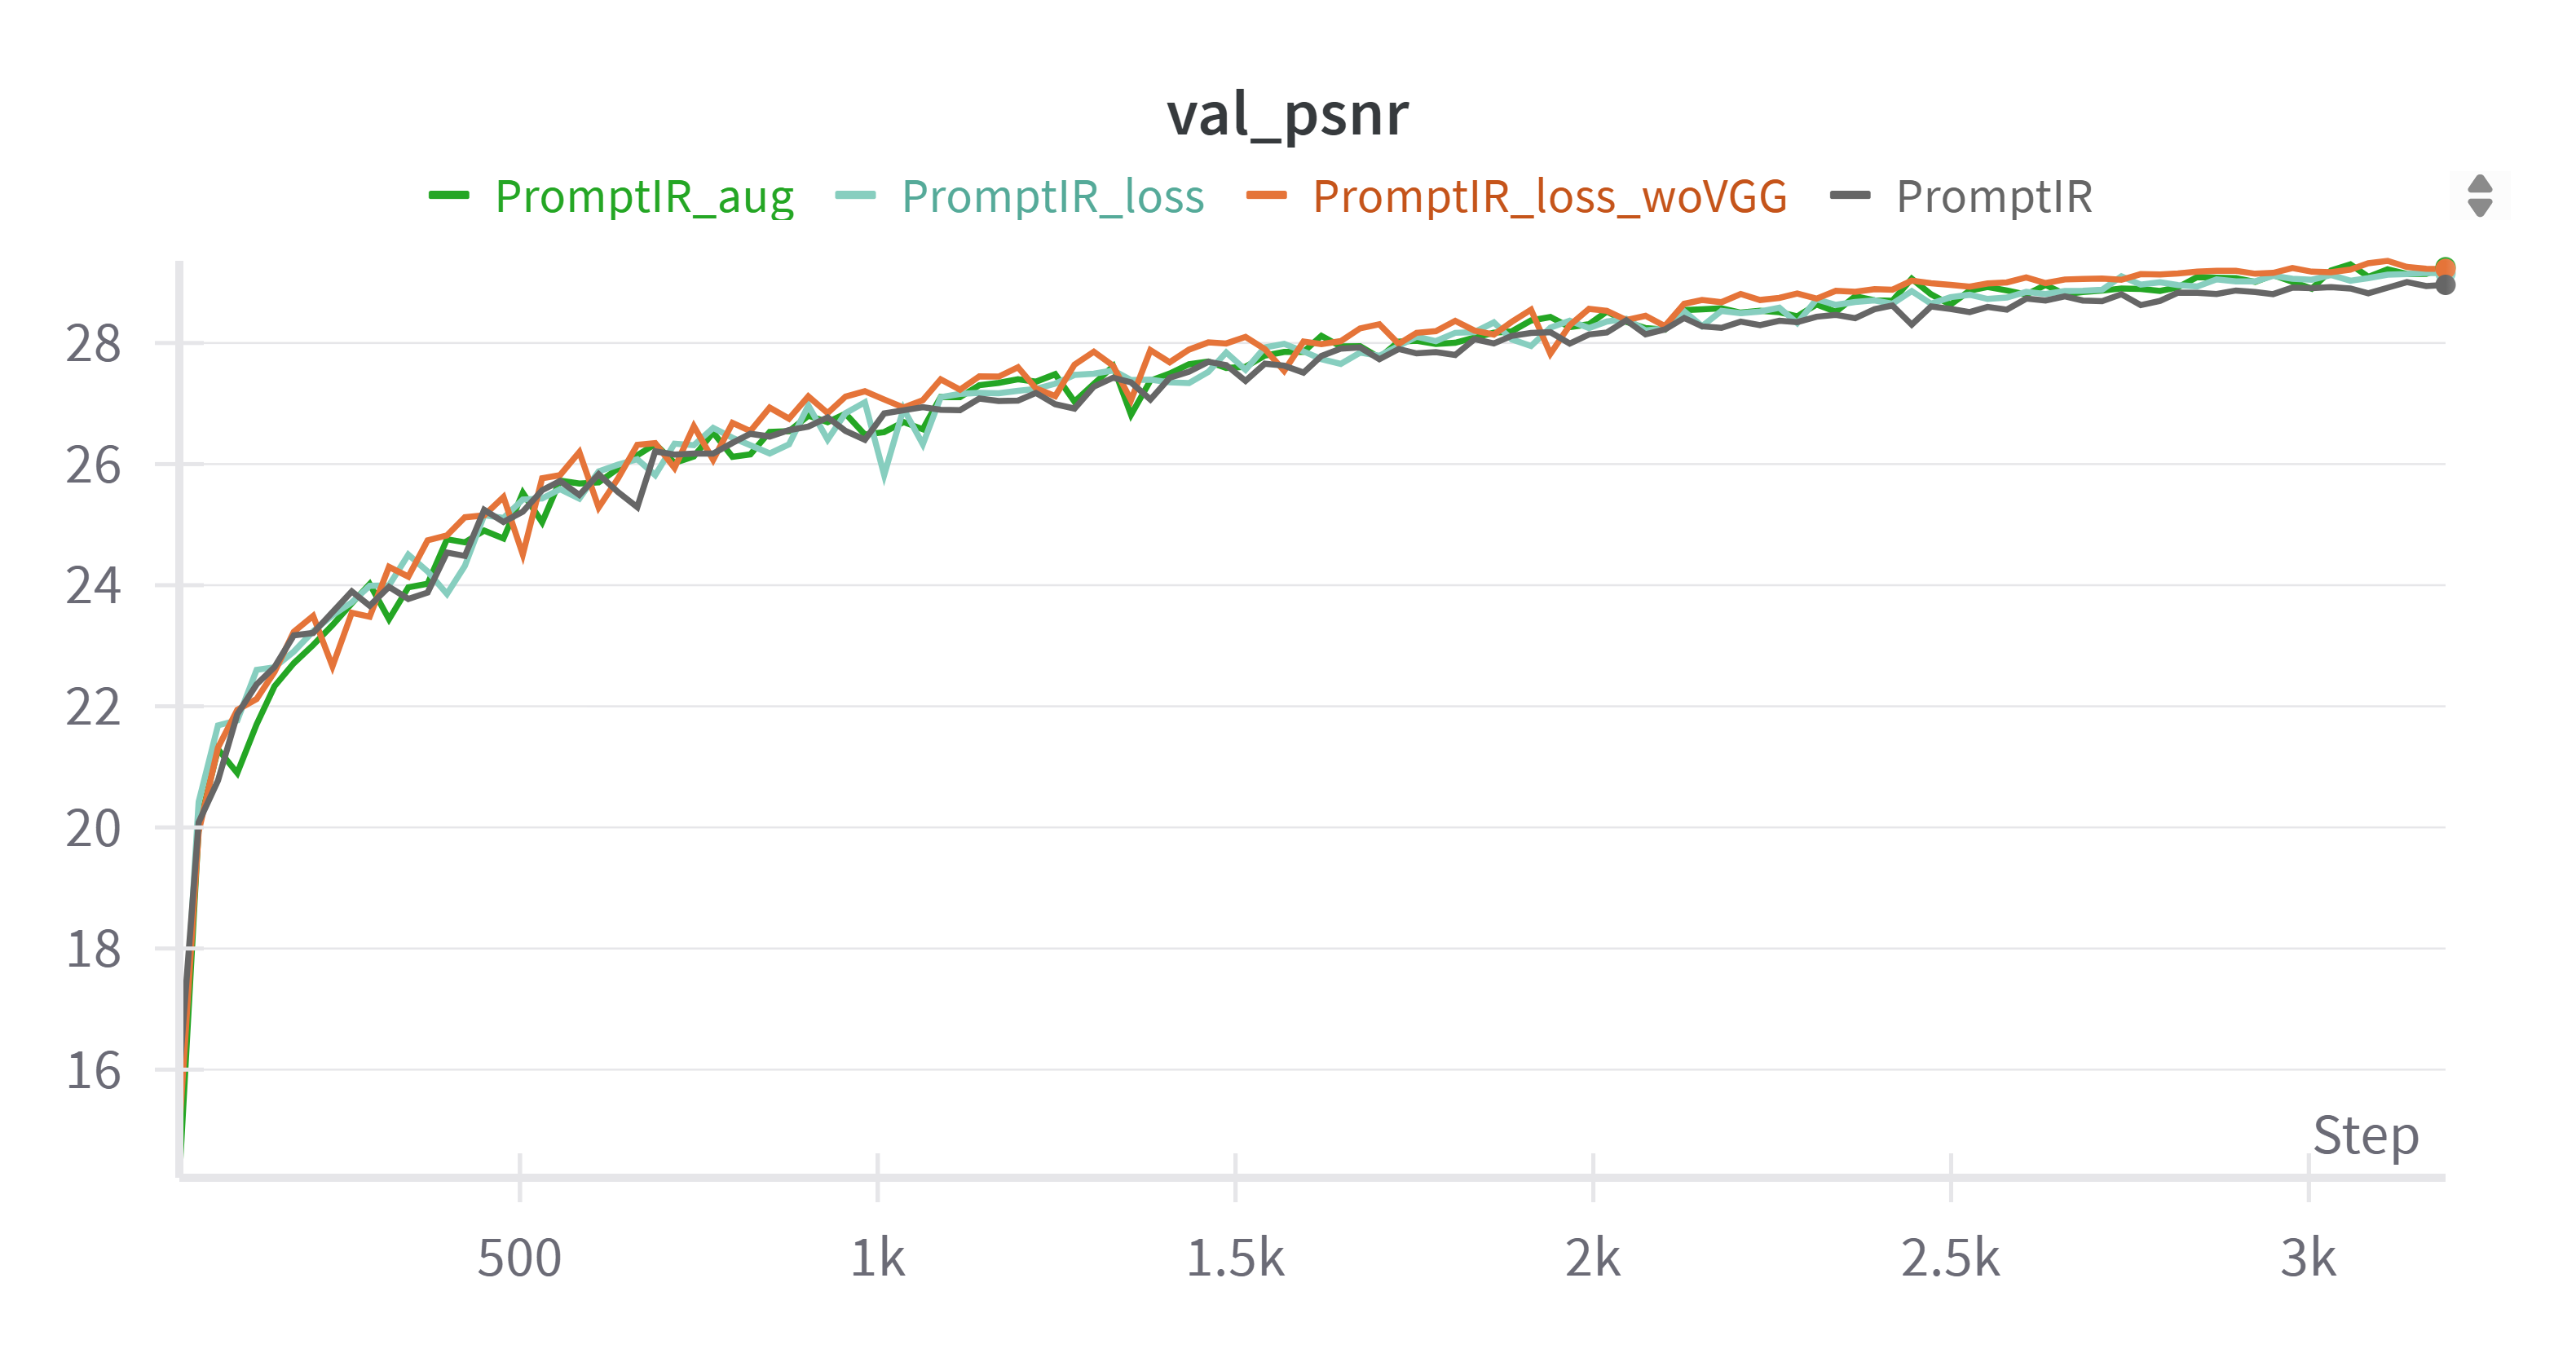
\includegraphics[width=0.95\linewidth]{assets/val_psnr.png}
  \caption{\textbf{Validation PSNR curve of different methods.}}
  \label{fig:val-psnr}
\end{figure}

\begin{figure}[h]
  \centering
  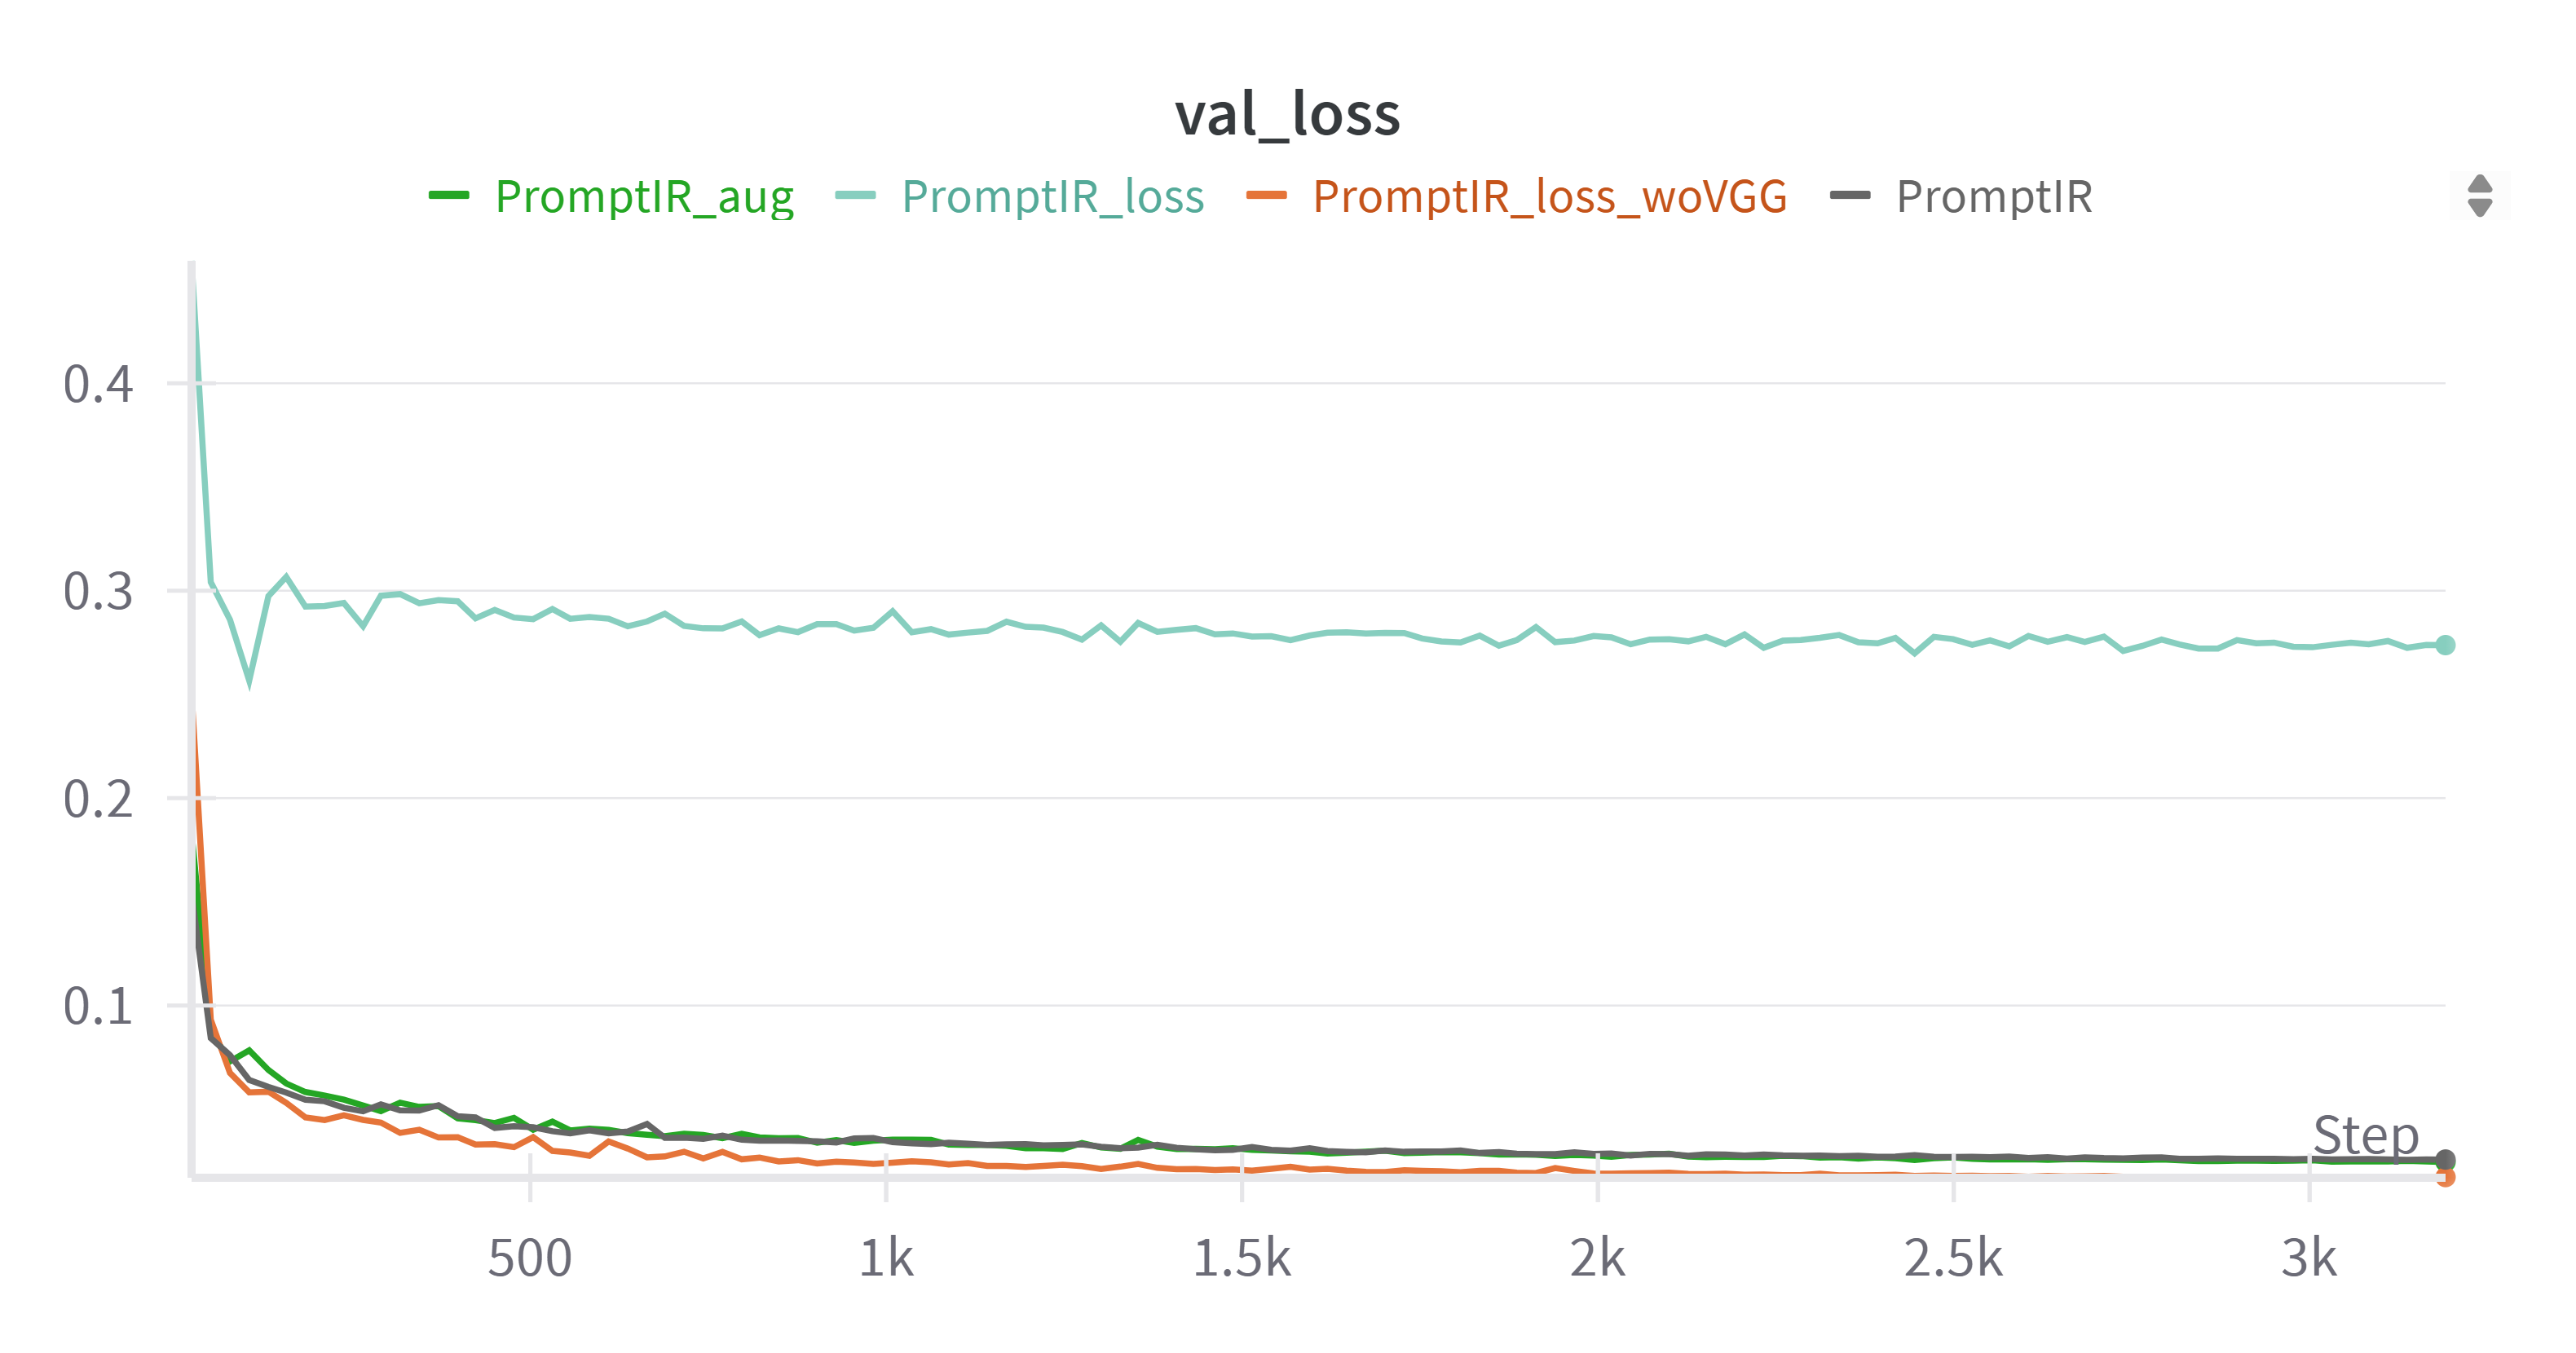
\includegraphics[width=0.95\linewidth]{assets/val_loss.png}
  \caption{\textbf{Validation loss curve of different methods.}}
  \label{fig:val-loss}
\end{figure}

\begin{figure}[h]
  \centering
  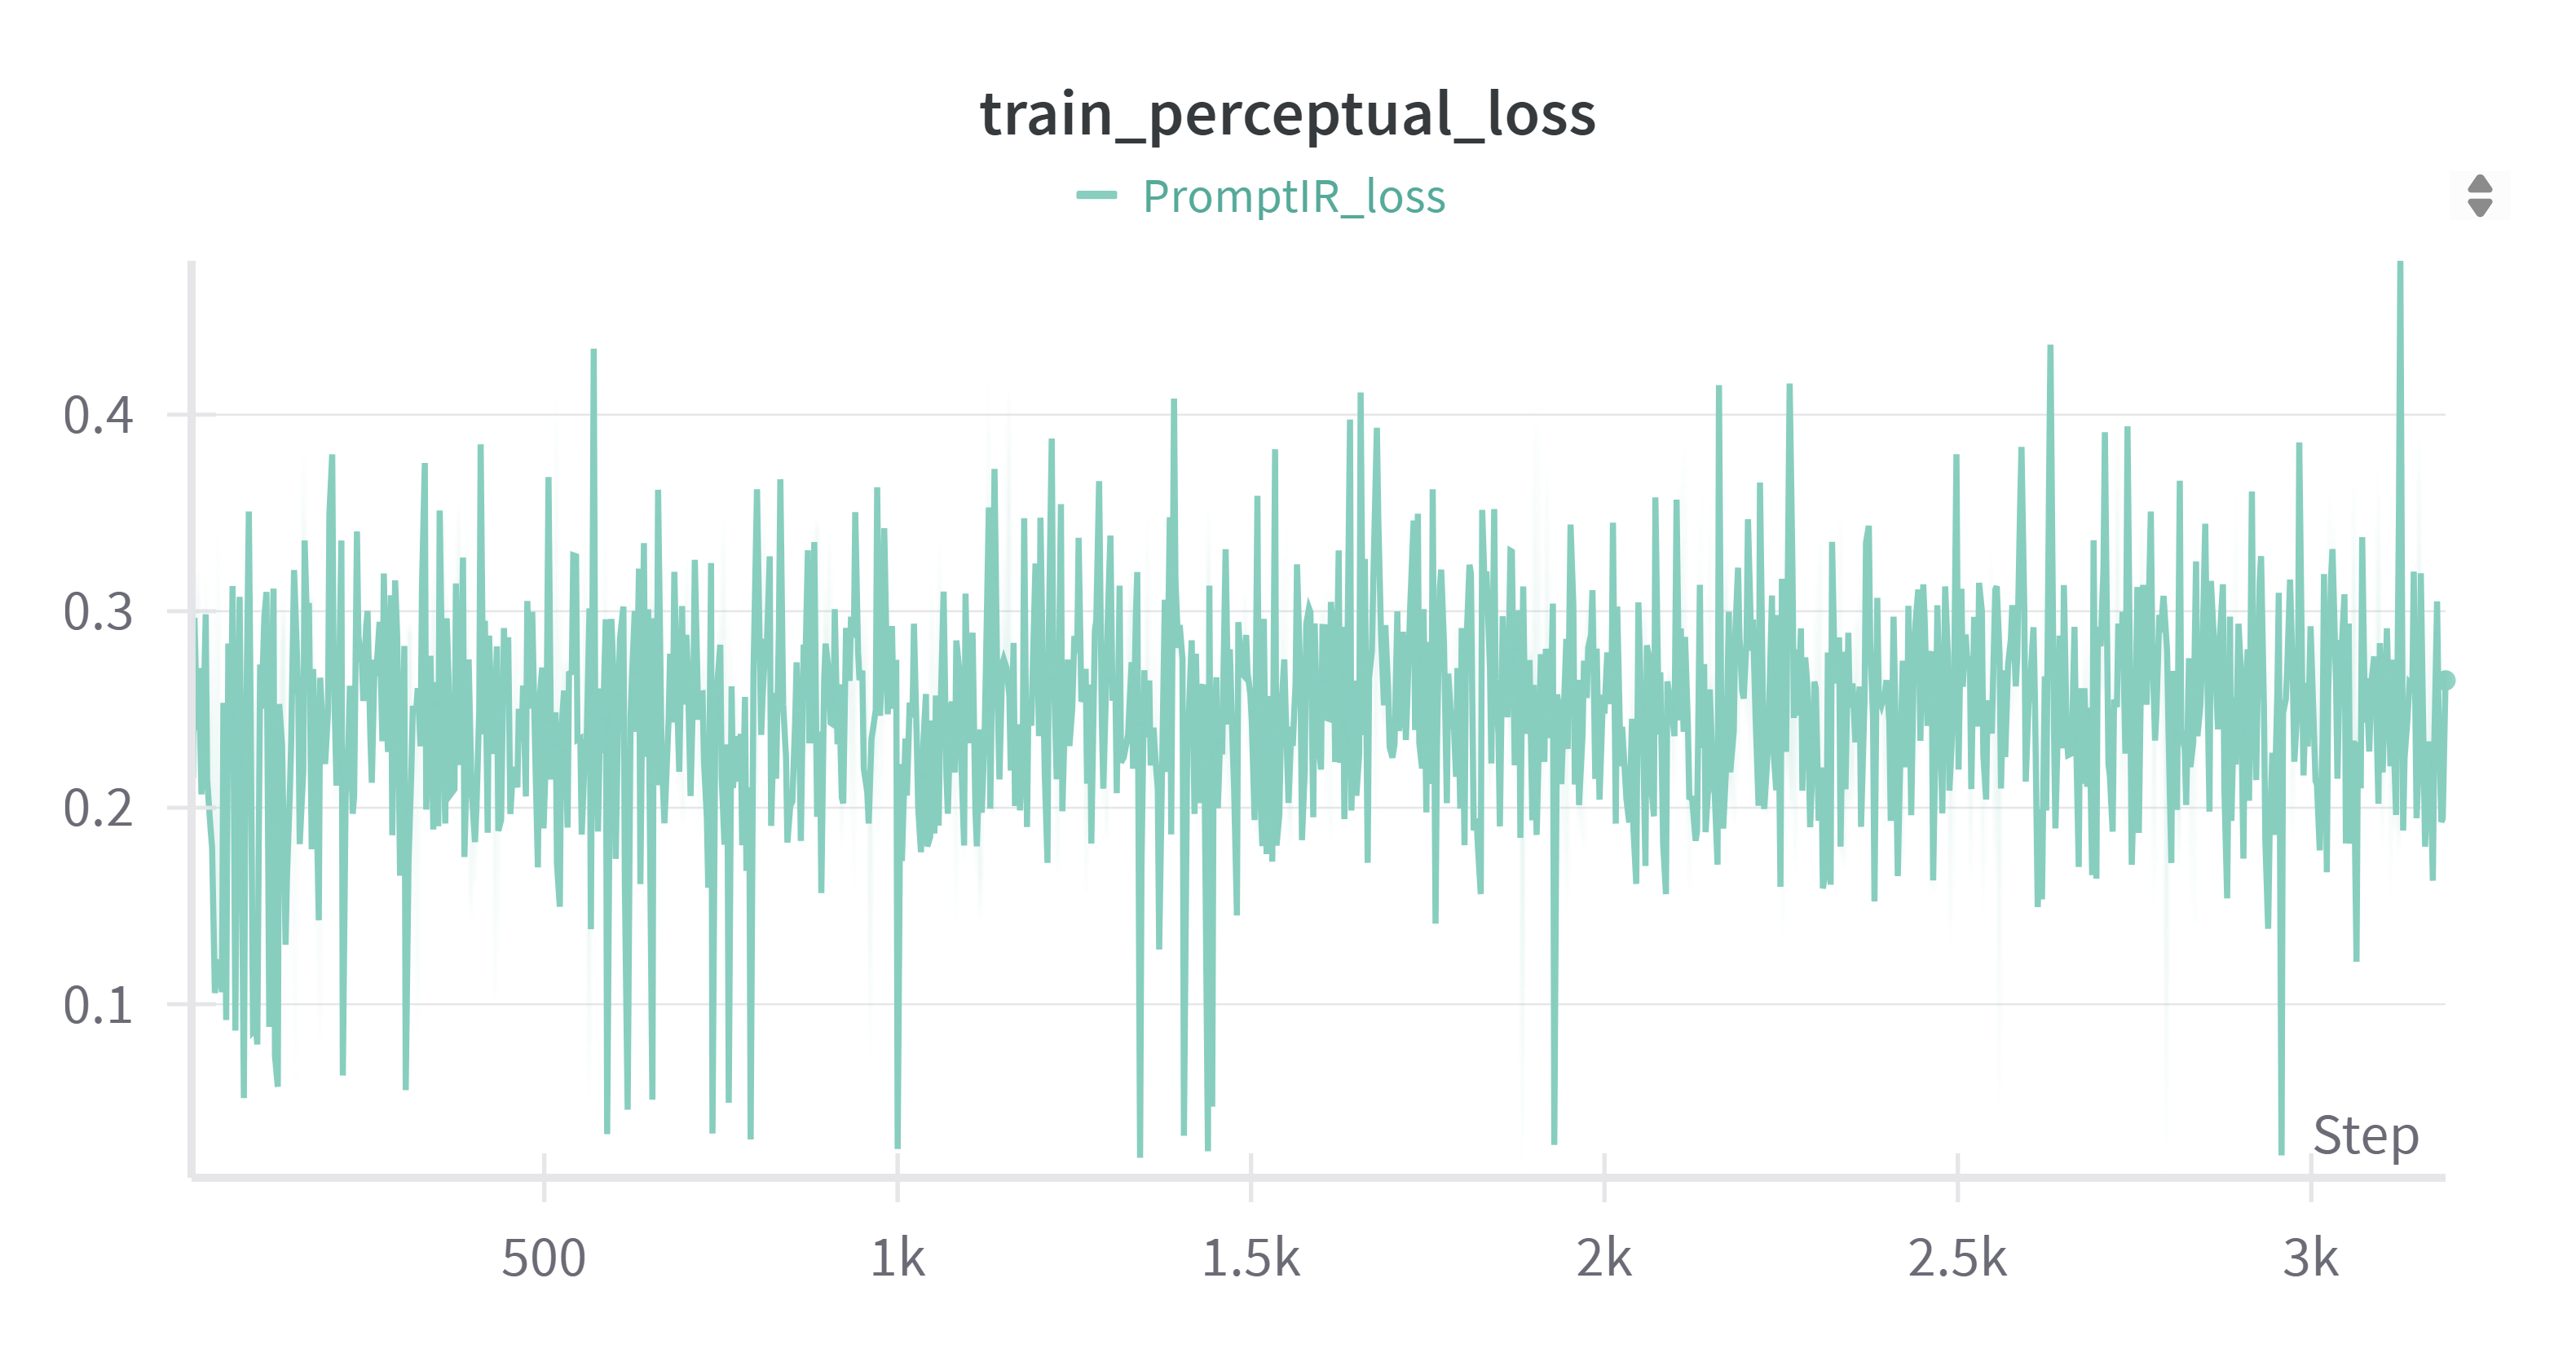
\includegraphics[width=0.95\linewidth]{assets/train_perceptual.png}
  \caption{\textbf{Validation perceptual loss curve for ``Loss''.}}
  \label{fig:val-perceptual}
\end{figure}

The visualization results of each method are shown in \cref{fig:result-derain}
and \cref{fig:result-desnow}. However, since the difference between each method
is not significant, it is recommended to see \cref{tab:result} to evaluate model
performance.

\begin{figure}[h]
  \centering
  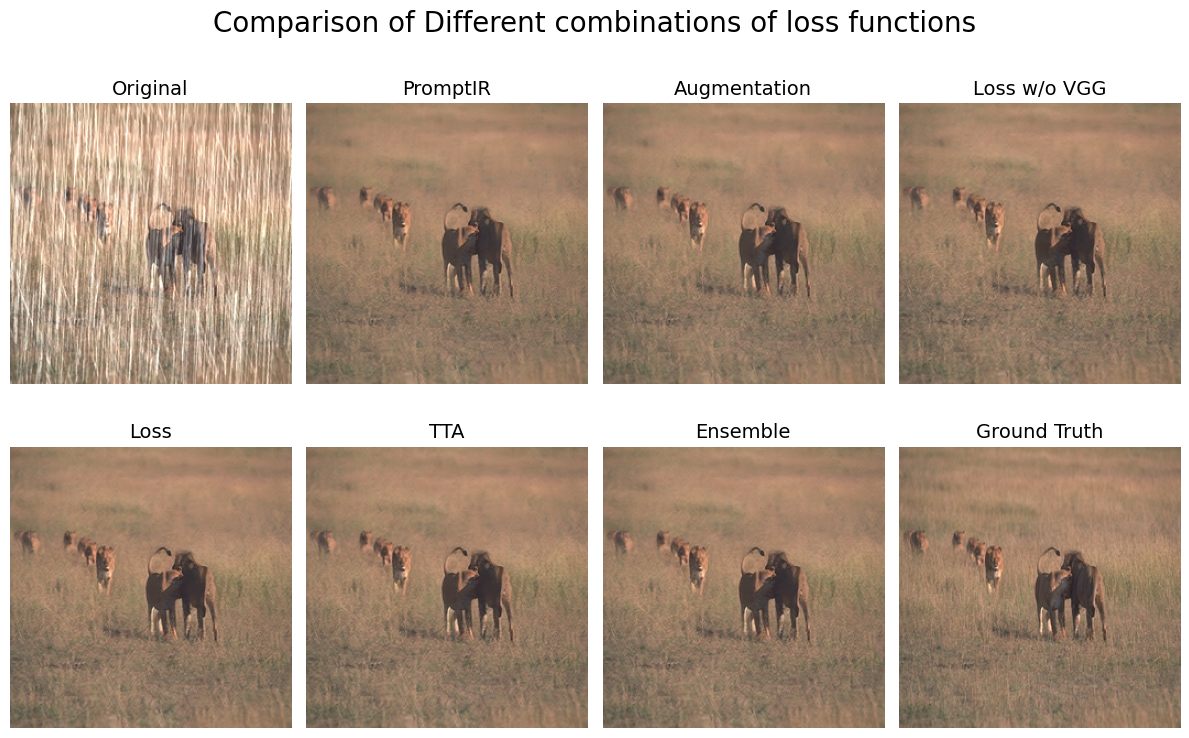
\includegraphics[width=0.95\linewidth]{assets/result-derain.png}
  \caption{\textbf{Visualization results of different methods in deraining task.}}
  \label{fig:result-derain}
\end{figure}

\begin{figure}[h]
  \centering
  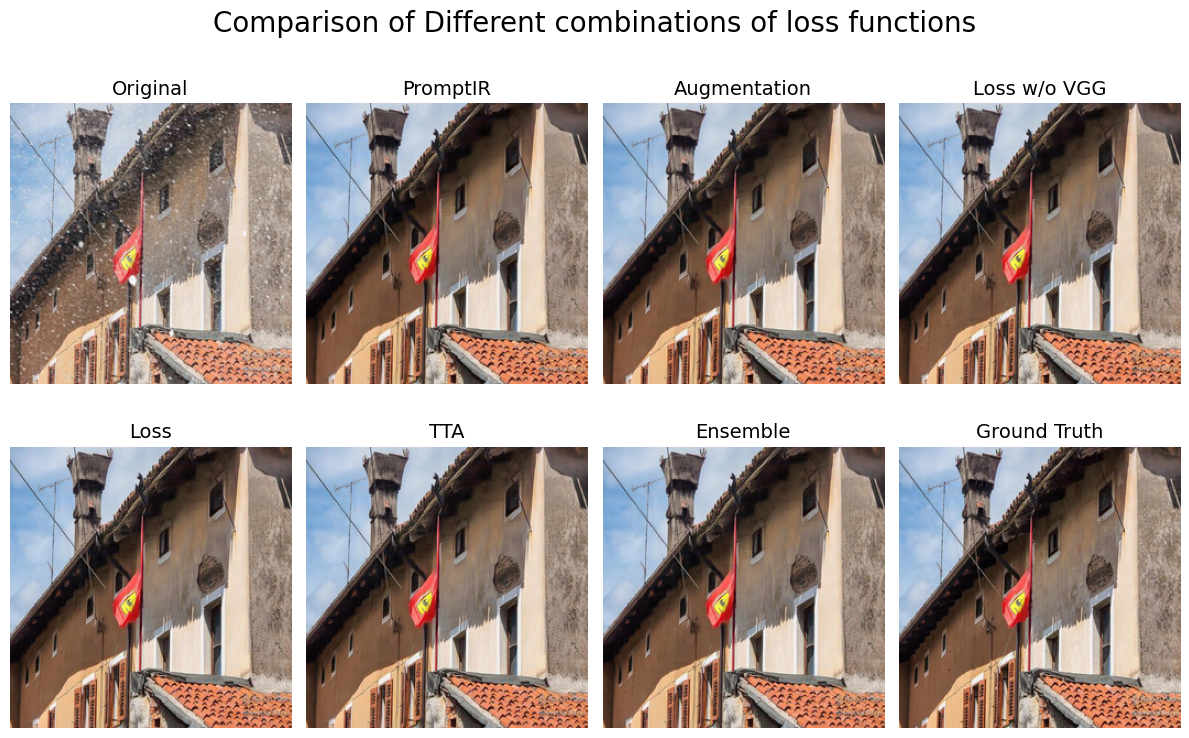
\includegraphics[width=0.95\linewidth]{assets/result-desnow.png}
  \caption{\textbf{Visualization results of different methods in desnowing task.}}
  \label{fig:result-desnow}
\end{figure}


% ----------------------- Other Experiments -----------------------

\section*{Other Experiments}
\label{sec:other-exp}

\subsection*{The Selection of Scheduler}

I've conducted experiments with different learning rate scheduler, including
Linear warmup cosine annealing, Cosine annealing warm restarts~\cite{CosineAnnealing},
and Cosine annealing. The results are shown in \cref{tab:scheduler} and visualized in
\cref{fig:scheduler}. Even though Warm restarts strategy performs better in validation
set (like previous homework), the Linear warmup cosine annealing performs better in
both public and private testing. Thus, it was chosen as the scheduler in the model.

\begin{table}[h]
  \centering
  \begin{tabular}{lccc}
    \toprule
    \multicolumn{1}{c}{\textbf{Method}}   & \textbf{Val}    & \textbf{Test pub.} & \textbf{Test priv.} \\
    \midrule
    Linear warmup                         & 28.9600          & \textbf{30.1508}    & \textbf{29.3773}  \\
    Warm restarts                         & \textbf{29.1132} & 29.8701             & 29.1540           \\
    Cosine annealing                      & 28.8869          & 29.8357             & 29.1742           \\ 
    \bottomrule
  \end{tabular}
  \caption{\textbf{The results of different scheduler.} PSNR is used as the
    evaluation metric as before. The highest values in each column are highlighted
    in bold.}
  \label{tab:scheduler}
\end{table}

\begin{figure}[h]
  \centering
  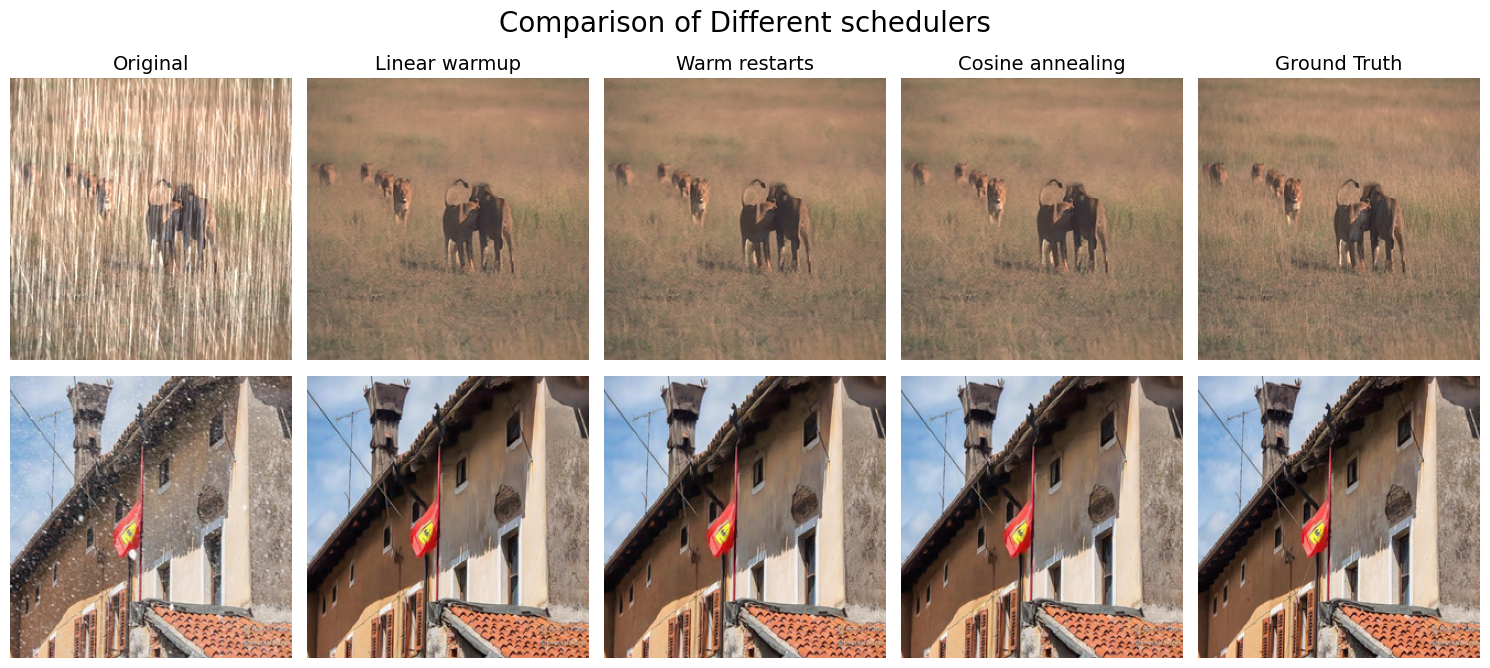
\includegraphics[width=1\linewidth]{assets/exp-scheduler.png}
  \caption{\textbf{Visualization results of different scheduler.}}
  \label{fig:scheduler}
\end{figure}

\subsection*{Loss Function}

Besides the loss functions mention in \cref{sec:method}, I also tried another loss,
color loss $\mathcal{L}_{\text{color}}$. This loss is calculated by converting
image to LAB color space and calculating the L1 loss between the predicted and
ground truth images in the A and B channels. The results are shown in
\cref{tab:loss} and \cref{fig:loss}.

\begin{table}[h]
  \centering
  \begin{tabular}{lccc}
    \toprule
    \multicolumn{1}{c}{\textbf{Method}}   & \textbf{Val}    & \textbf{Test pub.} & \textbf{Test priv.} \\
    \midrule
    L1 Loss (PromptIR)                    & 28.9600 & 30.1508 & 29.3773 \\
    $\mathcal{L}_{2} + \mathcal{L}_{\text{edge}}$ & \textbf{29.3570} & \textbf{30.2867} & 29.4772 \\
    $\mathcal{L}_{2} + \mathcal{L}_{\text{edge}} + \mathcal{L}_{\text{vgg}}$ & 29.1597 & 30.2547 & \textbf{29.5248} \\
    $\mathcal{L}_{2} + \mathcal{L}_{\text{egde}} + \mathcal{L}_{\text{color}}$ & 28.9432 & 29.8923 & 29.0913 \\
    \bottomrule
  \end{tabular}
  \caption{\textbf{The results of using different combination of loss function.}
    The highest values in each column are highlighted in bold.}
  \label{tab:loss}
\end{table}

\begin{figure}[h]
  \centering
  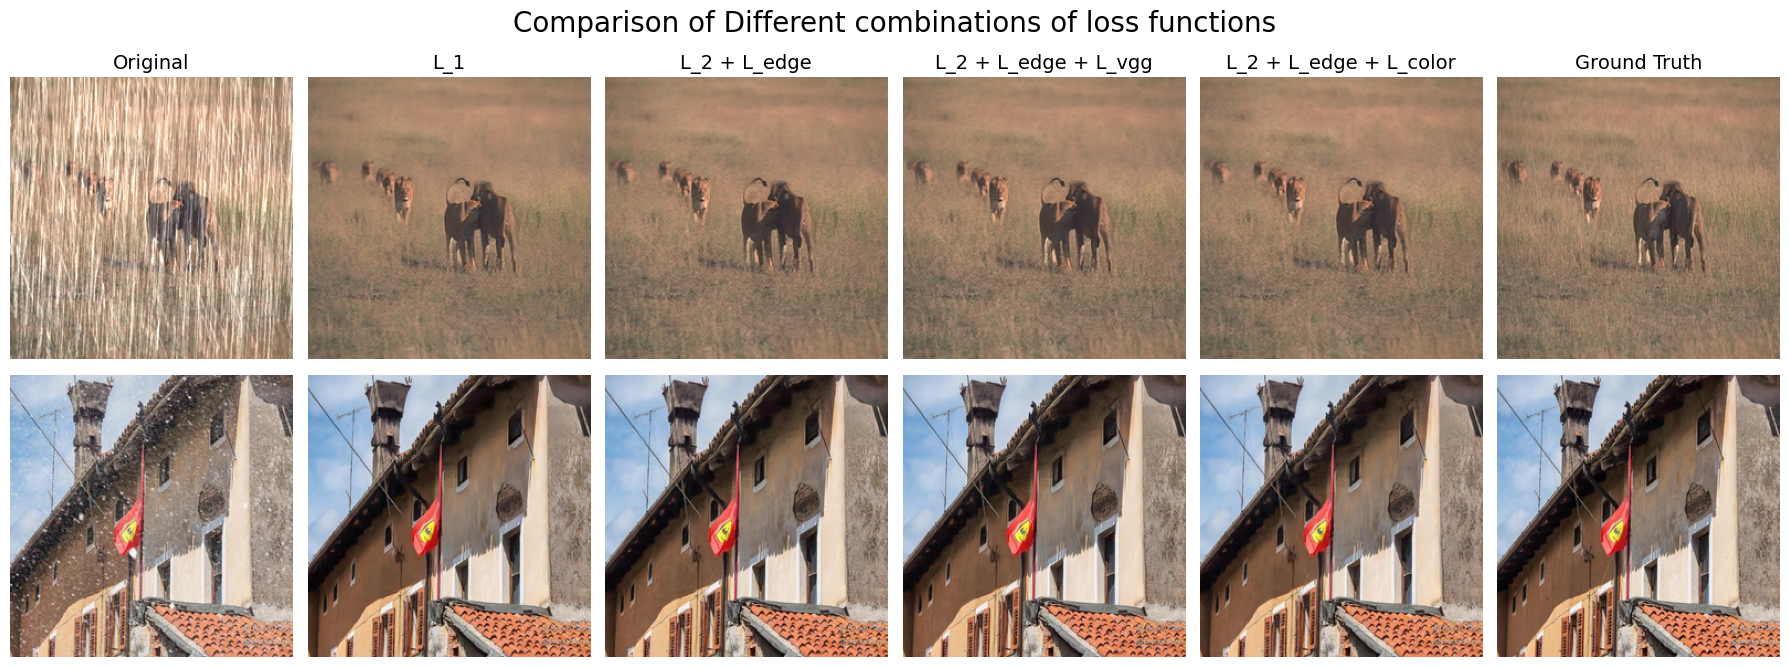
\includegraphics[width=1\linewidth]{assets/exp-loss.png}
  \caption{\textbf{Visualization results of diffenent loss functions.}}
  \label{fig:loss}
\end{figure}

I think it may help to recover the color more accurately, since I find that
PromptIR leads to some color distortion in the predicted images. However, adding
this color loss even degrades the performance of the model. Looking into the
value of color loss (\cref{fig:color-loss}), it seems not converged at all. It
just keeps fluctuating up and down. So I guess this loss may in turn disrupt the
optimization process.

\begin{figure}[h]
  \centering
  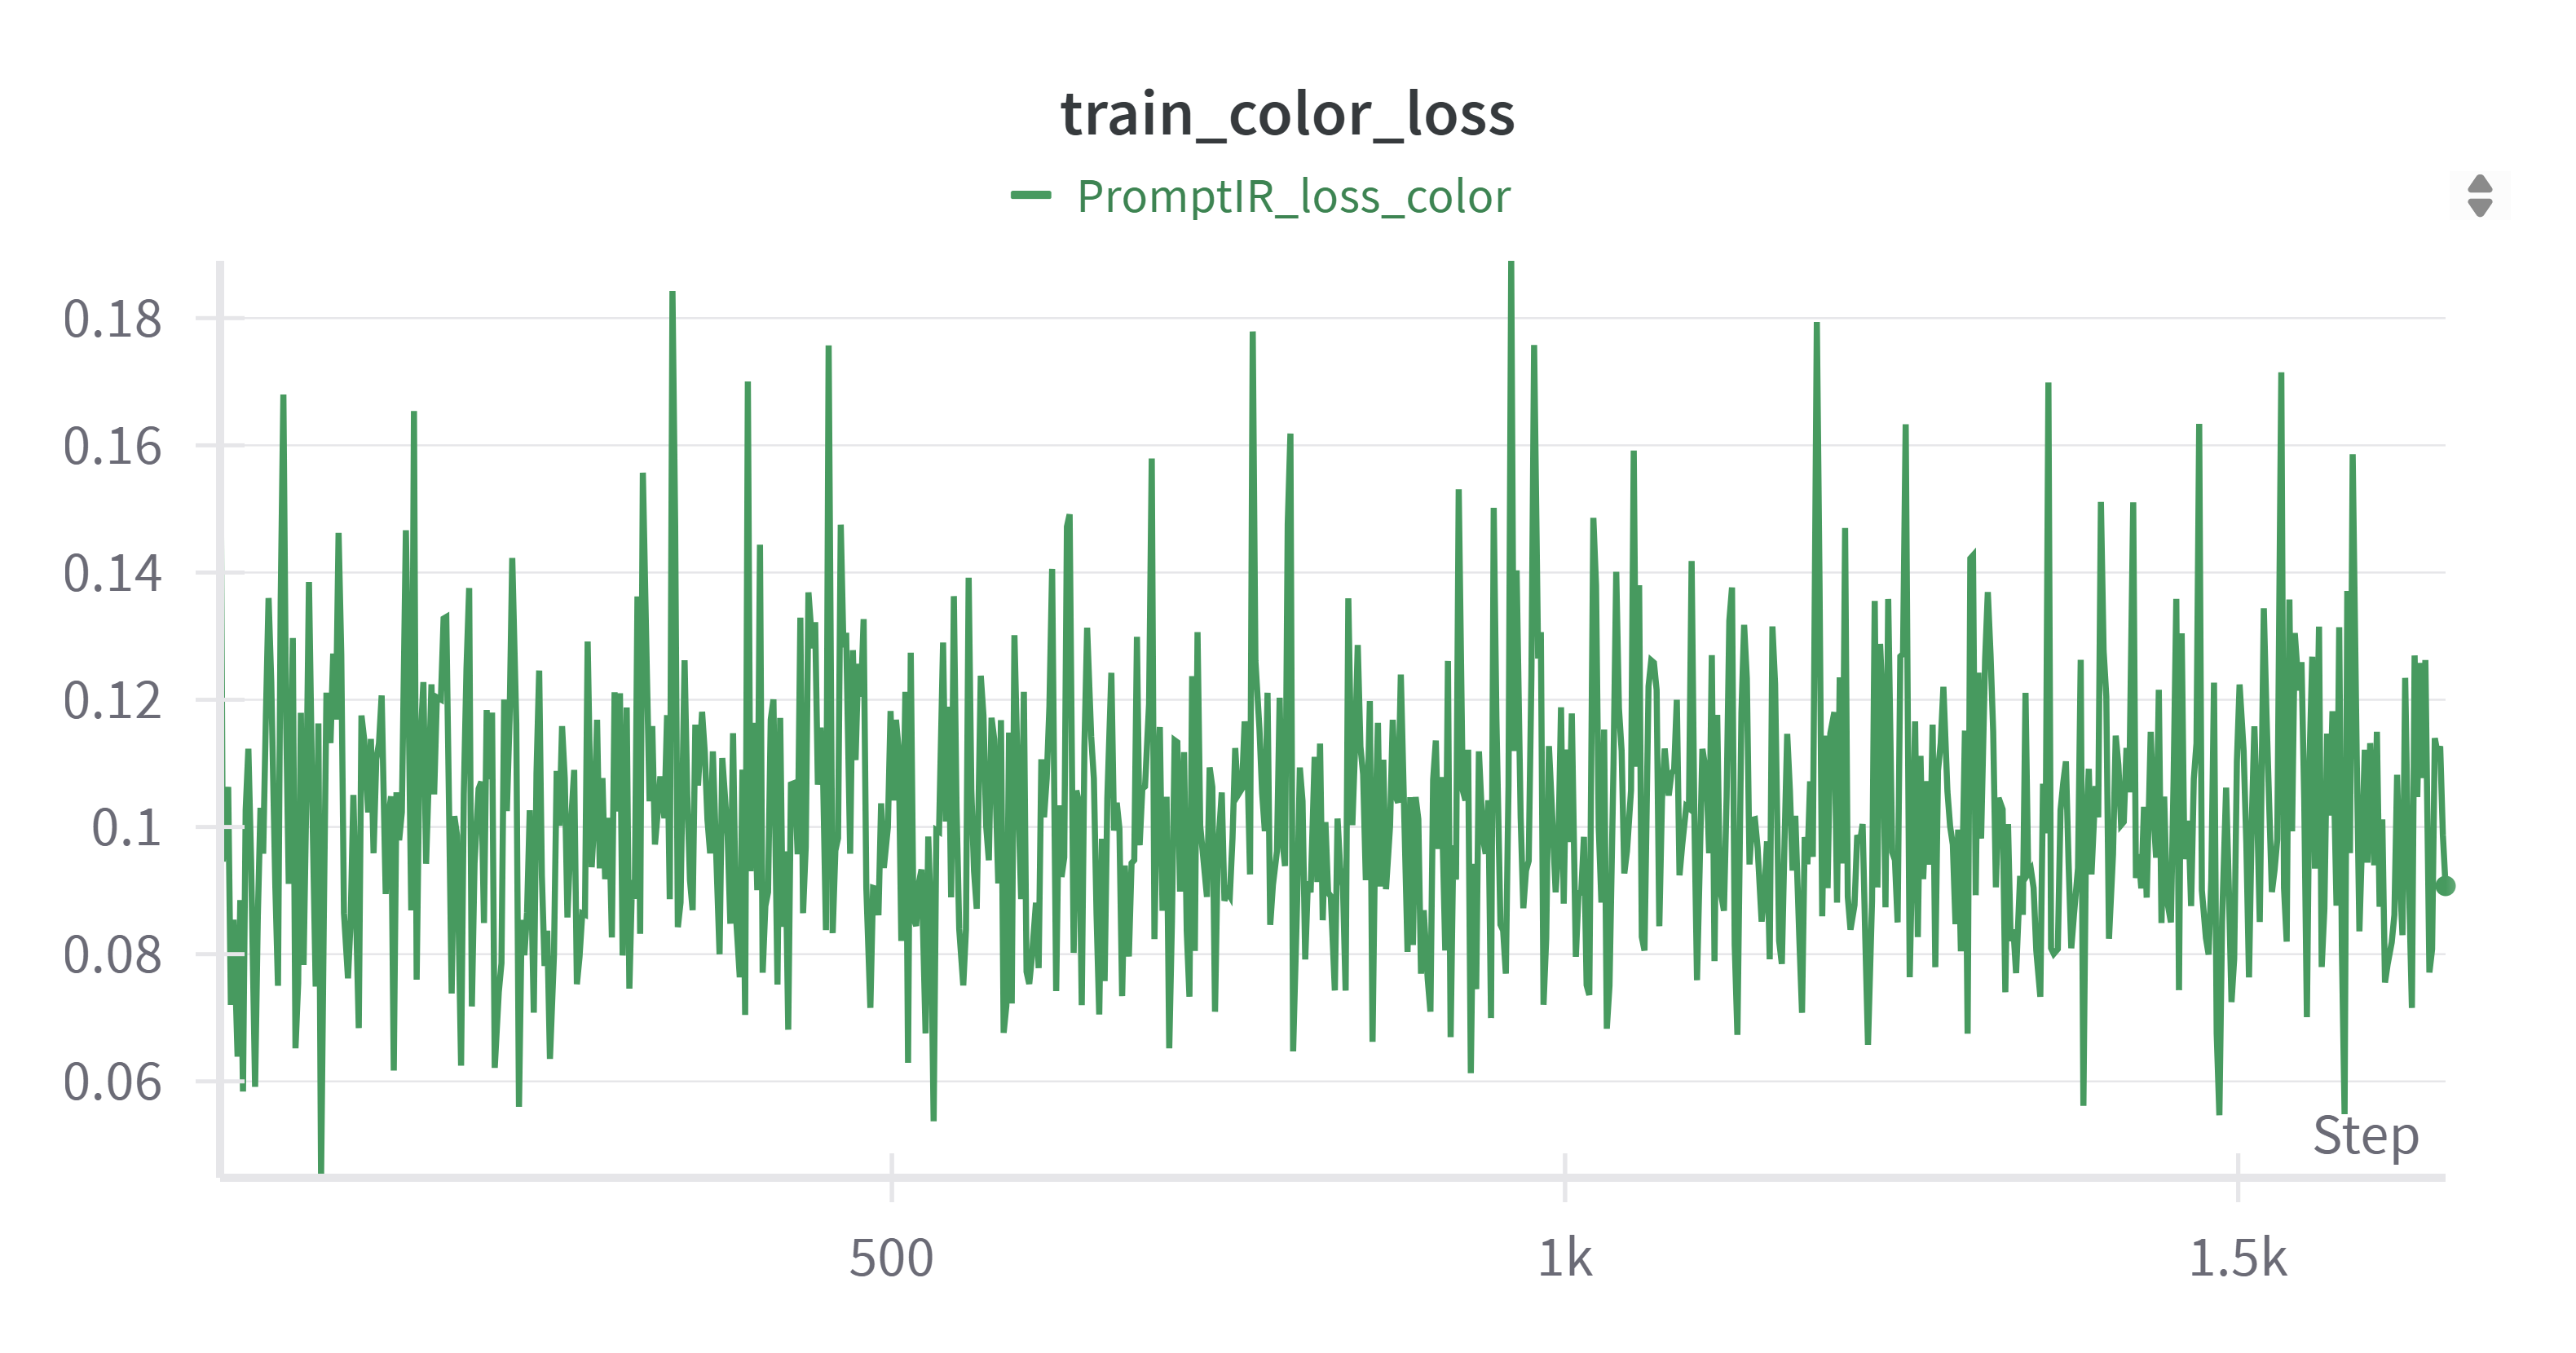
\includegraphics[width=1\linewidth]{assets/color-loss.png}
  \caption{\textbf{Color loss curve during training.}}
  \label{fig:color-loss}
\end{figure}


\subsection*{Model Architecture}

I've tried to modify the model architecture, including replacing the layer
normalization to bias free, and deleting the last transformer block (called
``refinement'' in their codebase). The results are shown in \cref{tab:arch}
and \cref{fig:arch}. Even though the model with bias free layer normalization
performs better in validation set, it drops its performance in testing set.
The final refinement transformer block is not mentioned in the original paper,
but it is used in the codebase. Removing this block may lead to the performance
drop, so it seems that this block can improve the performance of the model.
Thus, the layer normalization and refinement block are kept the same as the
original implementation.

\begin{table}[h]
  \centering
  \begin{tabular}{lccc}
    \toprule
    \multicolumn{1}{c}{\textbf{Method}} & \textbf{Val}     & \textbf{Test pub.} & \textbf{Test priv.} \\
    \midrule
    PromptIR                            & 28.9600          & \textbf{30.1508}    & \textbf{29.3773}   \\
    Bias free                           & \textbf{29.3065} & 30.0273             & 29.2934            \\
    No refinement                       & 28.8307          & 29.8706             & 29.1775            \\
    \bottomrule
  \end{tabular}
  \caption{\textbf{The results of different modification on model architecture.}
    The highest values in each column are highlighted in bold.}
  \label{tab:arch}
\end{table}

\begin{figure}[h]
  \centering
  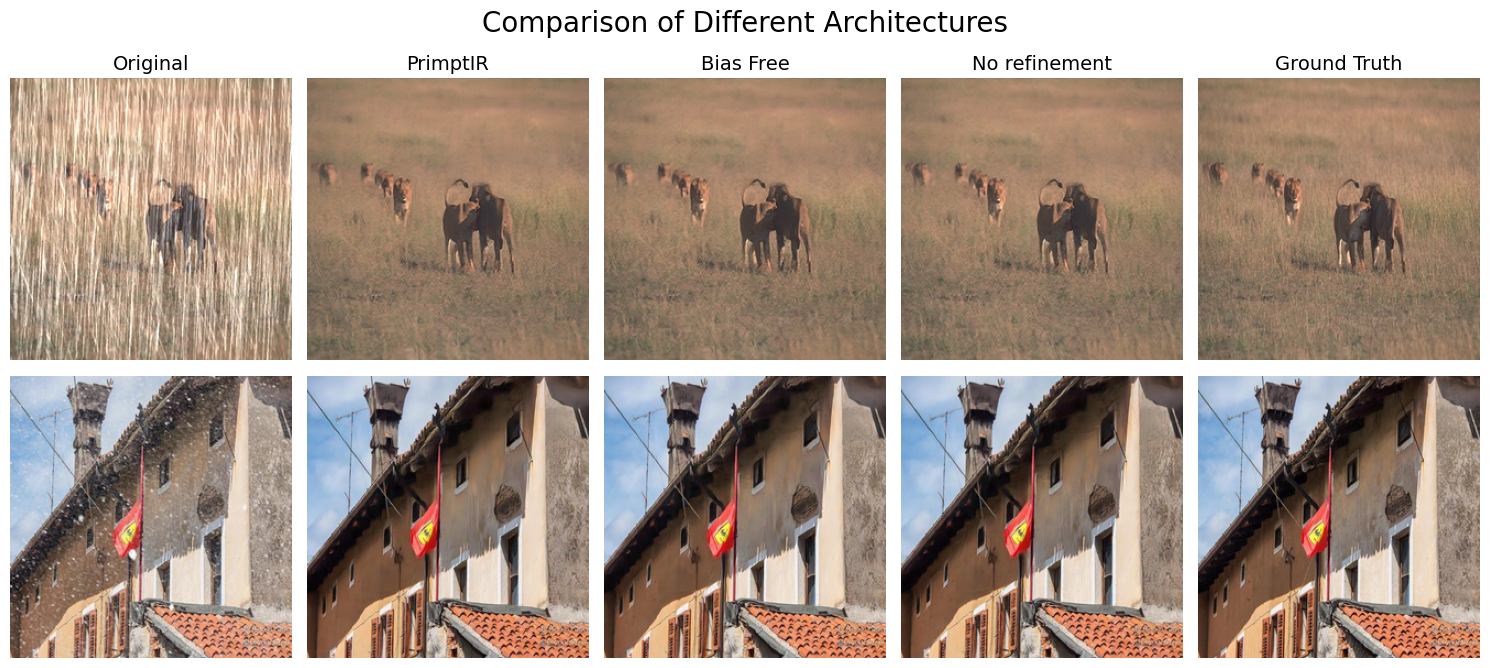
\includegraphics[width=1\linewidth]{assets/exp-arch.png}
  \caption{\textbf{Visualization results of different model architecture.}}
  \label{fig:arch}
\end{figure}


%%%%%%%%% REFERENCES %%%%%%%%%
{\small
\bibliographystyle{ieee_fullname}
\bibliography{egbib}
}

\end{document}